\documentclass{article}
\usepackage{fullpage,amsmath,amsthm,graphicx,enumitem,amsfonts}
\usepackage{multicol}
\usepackage{booktabs}
\usepackage{tikz}
\usepackage{xcolor}
\usepackage{cancel}
\newcommand{\tb}[1]{\textcolor{cyan}{[TB: #1]}}
\DeclareMathOperator*{\argmax}{arg\!\max}
\DeclareMathOperator*{\argmin}{arg\!\min}

\newcommand{\zs}[1]{{\color{blue}[ZS: #1]}}

\usepackage[normalem]{ulem} % only for \sout in \zsedit below
\newcommand{\zsedit}[2]{{\color{blue} \sout{#1}#2}}

\theoremstyle{definition}
\newtheorem{thm}{Theorem}
\newtheorem{question}[thm]{Question}
\newenvironment{solution}{\noindent\textit{Solution:}}{}

\title{ASEN 5264 Decision Making under Uncertainty\\
       Exam 2 (2026): POMDPs and Games}
\author{}


\begin{document}
\maketitle

\section*{SOLUTION}

\newpage
\section*{Question 1}
\begin{solution}
\textbf{a)}

If player one plays $G$, then player 2's possible payoffs are $G$: $R^2(G, G) = -2$ and $Y$: $R^2(G, Y) = 0$. Since the reward for playing $Y$ is greater, $Y$ is the only best response.

\textbf{b)}

The best responses can be denoted with the arrows:
\begin{itemize}
    \item Player 1: $(G,G) \rightarrow (Y,G)$
    \item Player 1: $(Y,Y) \rightarrow (G,Y)$
    \item Player 2: $(G,G) \rightarrow (G,Y)$
    \item Player 2: $(Y,Y) \rightarrow (Y,G)$
\end{itemize}
(students will likely draw arrows on the game diagram). Since \boxed{$(Y,G)$} and \boxed{$(G,Y)$} have no arrows leaving them (i.e. each is a best response to itself), they are pure Nash Equilibria.

Since there are three NE, there must be an additional mixed NE. In a mixed NE, players must be indifferent between their actions. In order for player 1 to be indifferent, player 2 must follow a policy that satisfies the following indifference equations:
\begin{align*}
    -2\pi^2(G) + 2 \pi^2(Y) &= u &\text{(Player 1 plays G)}\\
    0\pi^2(G) + 0\pi^2(Y) &= u &\text{(Player 1 plays Y)}\\
    \pi^2(G) + \pi^2(Y) &= 1 &
\end{align*}
Students may leave this unsolved, but it is easy to see that $u=0$ and $\boxed{\pi^2(G) = \pi^2(Y) = 0.5}$.

Similarly, player 1 must follow a policy that makes player 2 indifferent:
\begin{align*}
    -2\pi^1(G) + 2 \pi^1(Y) &= v &\text{(Player 2 plays G)}\\
    0 \pi^1(G) + 0 \pi^1(Y) &= v & \text{(Player 2 plays Y)}\\
    \pi^1(G) + \pi^1(Y) &= 1
\end{align*}
and we have $\boxed{\pi^1(G) = \pi^1(Y) = 0.5}$.

\textbf{c)}

A \textbf{Correlated equilibrium} would yield better results. In either of the pure Nash equilibria, one player receives payoff of 2, and the other 0, so it is unfair. In the mixed Nash equilibrium, the payoff is fair, but only 0. If we instead play the correlated equilibrium of $\pi(Y,G) = \pi(G,Y) = 1/2$, then each player has an expected payoff of 1. This could be implemented with a traffic light system that randomly chooses one car to go when cars approach either end.
\end{solution}


\newpage
\section*{Question 2}
\begin{solution}
\textbf{a)}
\begin{equation}
\begin{aligned}
    V^{\pi_C}(H) &= R(H,C) + \gamma \mathbb{E}_{o, s'}\left[R(s', \pi(o))\right] \\
    &= 4 + 1\sum_{s', o}T(s' | H, C) Z(o | C, s') R(s', \pi_C(o)) \\
    &= 4 + 1\left[0.90 \times 5 + 0.10 \times 0\right] \\
    &= 8.5
\end{aligned}
\end{equation}

\begin{equation}
\begin{aligned}
    V^{\pi_C}(D) &= R(D,C) + \gamma \mathbb{E}_{o, s'}\left[R(s', \pi(o))\right] \\
    &= -6 + 1\sum_{s', o}T(s' | D, C) Z(o | C, s') R(s', \pi_C(o)) \\
    &= -6 + 1\left[1 \times 0\right] \\
    &= -6
\end{aligned}
\end{equation}

\begin{equation}
    \boxed{\alpha^{\pi_C} = \begin{bmatrix}
        8.5 & -6
    \end{bmatrix}}
\end{equation}

\textbf{b,d)}

\begin{center}
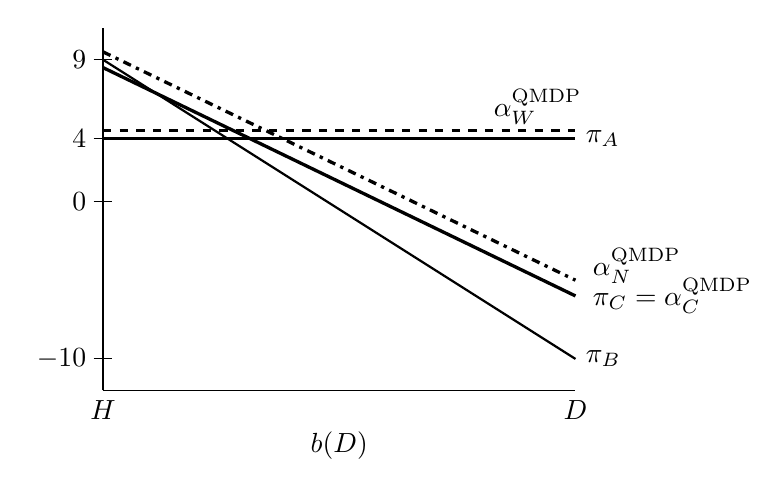
\begin{tikzpicture}[xscale=6, yscale=0.2]
    \draw (0,-12) -- (0,11);
    \draw (0,-12) -- (1,-12);

    \node[below] at (0,-12) {$H$};
    \node[below] at (1,-12) {$D$};
    \node[below=0.4cm] at (0.5,-12) {$b(D)$};

    \foreach \y in {-10,0,4,9} {
        \draw (-0.02,\y) -- (0.02,\y) node[left=6pt] {$\y$};
    }
    \draw[thick] (0,4) -- (1,4) node[right] {$\pi_A$};
    \draw[thick] (0,9) -- (1,-10) node[right] {$\pi_B$};

    \draw[very thick] (0,8.5) -- (1,-6);
    \node[anchor=west, fill=white, inner sep=1pt] at (1.03,-6.0)
        {$\pi_C = \alpha_C^{\mathrm{QMDP}}$};

    \draw[very thick,dashed] (0,4.5) -- (1,4.5);
    \node[anchor=west, fill=white, inner sep=1pt] at (0.82,6.0)
        {$\alpha_W^{\mathrm{QMDP}}$};

    \draw[very thick,dash dot] (0,9.5) -- (1,-5);
    \node[anchor=west, fill=white, inner sep=1pt] at (1.03,-4.1)
        {$\alpha_N^{\mathrm{QMDP}}$};
\end{tikzpicture}
\end{center}

\textbf{c)}
\begin{equation}
\begin{aligned}
    Q^{\text{MDP}}(s,a) & = R(s,a)+\gamma \sum_{s'}T(s'| s,a)\max_{a'}R(s',a') \\
    Q^{\text{MDP}}(H,N) &= 5 + \gamma \left[0.90 \times 5 + 0.10 \times 0\right] \\
    &= \boxed{9.5}
\end{aligned}
\end{equation}


\textbf{e)}
QMDP 2-step pseudo-alpha vectors assume full state revelation following the action. This is exactly what happens with the \textbf{C}heck action, so the 2-step QMDP value is identical to that of $\pi_C$. QMDP 2-step pseudo-alpha vectors, when doing max backups, serve as an upper bound on the value achievable by an observation-dependent POMDP conditional plan. Furthermore with a POMDP conditional plan, you would take the check action to resolve state uncertainty, but with QMDP alpha vectors, one would never check.



\end{solution}


\newpage
\section*{Question 3}
\begin{solution}

\textbf{a)}
The best response can be solved as a single-agent MDP with marginalization
\[
\tilde{T}(s'|s,a^1) = \sum_{a^2} \pi^2(a^2 | s ) T(s' |s, a^1, a^2)
\]
\[
\tilde{R}(s|a^1) = \sum_{a^2} \pi^2(a^2 | s )R(s, a^1, a^2)
\]
with $S$ and $\gamma$ remaining the same and only the action space for the first player used. This MDP, $(S, A^1, \tilde{T}, \tilde{R}, \gamma)$, can be solved with an algorithm such as policy iteration to find the best response.



\textbf{b)}

This is iterated best response (IBR) and is \emph{not} guaranteed to reach a Nash equilibrium policy. For example, in the Rock-Paper-Scizzors game (a 1-state Markov Game), the best responses will continue to cycle forever.

\textbf{c)}


To prove that this is not a Nash equilibrium, you should use matrix-based policy evaluation to calculate the values for both players for the joint policy, $$U^1(\pi^1, \pi^2) \text{ and } U^2(\pi^1, \pi^2).$$ Then, calculate best responses for both players and the utilities, $$U^1(\mathbf{BR}(\pi^2), \pi^2) \text{ and } U^2(\pi^1, \mathbf{BR}(\pi^1)).$$ If $U^1(\mathbf{BR}(\pi^2), \pi^2) > U^1(\pi^1, \pi^2)$ or $U^2(\pi^1, \mathbf{BR}(\pi^1)) > U^2(\pi^1, \pi^2)$, then $(\pi^1, \pi^2)$ is not a NE because at least one of the players is not playing a best response.

If the best response utilities are equal to the original utilities, then $(\pi^1, \pi^2)$ is an NE.


\end{solution}

\end{document}
